\chapter{Interferometric preparation uncertainty}\label{chap:interferometric_prep_ur}

\section{Introduction} 

In this section we seek to apply the concepts considered in section \ref{chap:low_dim_prep} to an infinite dimensional system. Although the setup we consider is reasonably simple, the generalisation requires attention so some mathematical subtleties which are not features of the finite dimensional case. One of these subtleties arises because we will be interested in cases for which it is not sufficient to consider the outcome set to be a simple subset of $\R$. In particular there are cases where there is not a natural definition for the ``mean'' of a probability distribution, nonetheless we may employ the methods of \ref{sec:comp-measures-and-dists} to categorise probability measures over arbitrary metric spaces.

We consider a (nonrelativistic) massive particle moving on a two-dimensional plane, perpendicularly incident on an infinite aperture $A$, capable of partially measuring the particle's transverse position (the ``path'' in an interference experiment), in the sense described below. Alternatively, we remove $A$ and instead place another position detector $B$ beyond $A$ at a distance large 
%The beam is incident on the infinite aperture with identical slits placed at unit distance from each other, so that each interval $n + [-1/2, 1/2]$ contains one slit, described by the subinterval $n+ I$ where $I\subset [-1/2, 1/2]$ is a fixed interval. Passage of through the aperture mask is then modelled (up to normalisation) by the projection
%$$
%\psi \mapsto Q_A\psi
%$$
%where $Q_A$ is the projection onto the whole infinite aperture $A= \cup_{n} (n+I)\subset \mathbb R$. The subset of particles passing through the aperture is described by the resulting conditional quantum state $Q_A\psi$, in general an arbitrary element of $L^2(A)$ (considered as a subspace of $L^2(\R)$). The particles then proceed freely until they encounter an (infinite) planar detector, where the interference pattern is measured.
enough so that the Fraunhofer approximation becomes valid, that is, late-time position measurement asymptotically corresponds to a momentum measurement. An explicit calculation of the asymptotic form of the free evolution suitable for the present setup was included in \cite{BB2013}; for a more detailed proof, see e.g. \cite[Theorem IX.31]{RSII}. Hence, up to scaling of units (which we will not explicitly indicate), the free evolution between the two position detectors is simply approximated by the Fourier-Plancherel transform $\mathcal F$, and position observable in the second detector is essentially equal to momentum in the position space of the first detector.

\subsection{Topology of the outcome sets for the interferometric observables}

Hence one is lead to the idea that position and momentum observables describe the path and interference measurements, respectively. However, interferometry does not yet feature in this setting in any way - we need to constrain the detectors in a suitable way. We do this by assuming a periodic structure on the \emph{second} detector, in accordance with the idea that it should display the interference pattern. A suitable way of formulating this assumption is to observe the transverse location of the particle modulo some fixed period, which (up to a choice of units) can be taken $[-\pi,\pi]$. Now the subsequent development depends crucially on the topology we choose on this interval - in fact, there are two natural choices:
\begin{itemize}
\item[(a)] the topology of a circle $\mathbb T$ (i.e. identify the endpoints), and
\item[(b)] the relative topology coming from $\mathbb R$ (with endpoints distinct).
\end{itemize}
With this distinction in mind, we can now discuss the outcome sets of the ``path'' observable. In case (a) the natural choice is the topological dual group of $\mathbb T$, that is the set of integers $\mathbb Z$, while in case (a) one would take the dual of $\mathbb R$, which is just $\mathbb R$.

In order to quantify uncertainty in these outcome sets, we need to specify suitable metrics, which will then have to be compatible with the topologies in the two cases (a) and (b). For the circle there are two natural choices: distance across the disc and along the circle. Both can be written in the form $d(\theta,\theta')^2 = V(\theta-\theta')$ where $V$ is a periodic, symmetric and continuous function on $\mathbb R$, with periodicity interval $[-\pi,\pi]$. We will restrict to the case $V(\theta) = \theta^2$, extended periodically outside $[-\pi,\pi]$. For $\mathbb R$ and the interval $[-\pi,\pi]$ with the relative topology, we take the usual metric $d(x,y)^2=(x-y)^2$.

Having fixed a metric we will use the $\alpha$-deviation defined in \eqref{eqn:wassersten-variance} to measure the uncertainty. We will focus on the case $\alpha=2$, which matches the usual variance when the metric $d$ is the Euclidian distance on $\R$. On the other hand the circle is not a (topological) subspace of $\R$, so the standard variance will not suffice in that case.

\subsection{Interferometric observables}

We begin by fixing the interference pattern measurement to be the simplest possible one compatible with the periodic structure described above - describing position modulo $2\pi$, with basic periodicity interval $[-\pi,\pi]$. This is the operator $\MOD P$ acting in the momentum space as
\begin{align}
(\MOD P\hat\psi)(p) = (p-2\pi n)\hat\psi(p), \text{ for } p\in [-\pi,\pi] +2\pi n,
\end{align}
where $n\in \mathbb Z$ and $\hat \psi$ denotes the Fourier transform. This operator was called \emph{modular momentum} by Aharonov et al \cite{aharonov-modular-variables}, and investigated subsequently in \cite{PhysRevA.90.022115}.

The question is then what should be the corresponding path measurement. In order to incorporate both cases (a) and (b) we need to go somewhat beyond the above cited literature. The path measurement in the interferometric setting is expected to be complementary to the interference pattern measurement $\MOD P$. We consider ``complementarity" in the straightforward sense of ``canonically conjugate'', formulated mathematically through covariance (see \cite{Kiukas2019} for a review of the meanings of complementarity in quantum mechanics). That is, the conjugate path observable $E$ should transform covariantly under the shifts generated by $\MOD P$: for the cases (a) and (b), respectively, we require
\begin{align}
e^{-im \MOD P}E_ne^{im \MOD P} &= E_{n+m}, \,n,m\in \mathbb Z, \label{covA}\\
e^{-ix \MOD P}E(X)e^{ix \MOD P} &= E(X+x), \,X\subset \mathbb R,\,x\in \mathbb R. \label{covB}
\end{align}
In both cases, there are plenty of observables satisfying the requirement. In order to find a suitable canonical choice it makes sense to require that the path measurement be optimal in some sense. There are various notions of optimality, most of which are related to having minimal amount of noise. For the present situation, a suggestive choice of is to restrict to \emph{variance-free} observables, that is, to those whose intrinsic noise is minimal. Below we consider this restriction in the two relevant cases.

%$$
%Q_A\psi \mapsto \widehat{Q_A\psi},
%$$
%Now prototypical states that respect the periodic structure of the aperture are of the form
%\begin{equation}\label{basicstates}
%\psi(x) = \sum_{n\in Z} c_n \phi(x-n),
%\end{equation}
%where $\phi\in L^2(I)\subset L^2[-1/2,1/2]$ and $(c_n)$ is such that $\sum_{n}|c_n|^2 = 1$. In other words, a direct sum of copies of one wave function supported in one periodicity interval of the aperture, modulated by the coefficients $c_n$. For such a wave function the result of the above two operations is
%$$
%\widehat{Q_A\psi}(p) = \eta(p)\widehat\phi,
%$$
%where $\eta$ is the Fourier series with coefficients $c_n$, that is, $\eta(p) = \frac{1}{\sqrt{2\pi}} \sum_{n\in \mathbb Z} c_n e^{inp}$, which is again periodic but with the inverse period $2\pi$.


% \subsection{Measuring uncertainty}
% \label{subsec:defining-uncertainty-measure}

% We will measure the uncertainty using the $\alpha$-deviation defined in , although this is defined arbitrary $\alpha$ we will focus on the case $\alpha=2$, because this makes the link to the usual variance most apparent. Indeed, for probability measures where the variance exists the $2$-deviation is exactly the variance.

% Explicitly we will characterise two preparation uncertainty regions, defined by the $2$-deviation

% For the purpose of exposition we first consider the probability measures defined on the (unit) circle $\T \defeq \faktor{[-\pi,\pi]}{\sim}$, where $\sim$ identifies the points $-\pi$ and $\pi$. We give $\T$ the structure of a metric space, by defining
% \begin{align}
%   d(x_1,x_2) \defeq \min_{n\in \{-1,0,1\}} \abs{x_1 + 2n\pi - x_2},
% \end{align}
% where the minimisation reflects the fact that two points may be connected by arcs either way around the circle. We note that there can be no analogue of the first moment of a probability measure in this setting, for example because there is no natural way to assign a unique ``mean'' to the uniform measure. Nonetheless we can define a measure of uncertainty which generalises the variance. For a general metric space $(\mathsf A,d)$, real $\alpha\geq 1$, and Borel probability measure $\mu$ we define
% \begin{align}
%   \ws{\mu}[\alpha]^\alpha \defeq \inf_{x_0} \int_{\mathsf{A}} d(x,x_0)^\alpha d\mu(x),
% \end{align}
% noting that since the measure is Borel, and the integrand is non-negative, the integral exists, but may be infinite for some choices of $\alpha$ and $\mu$ if $(\mathsf{A}, d)$ is not bounded. We define the usual Wasserstein $\alpha$-distance between two probability measures on $(\mathsf A,d)$
% \begin{align}
%   \ws{\mu,\nu}[\alpha]^\alpha  \defeq \inf_{\gamma\in\Gamma(\mu,\nu)} \int_{\mathsf{A}\times\mathsf{A}} d(x,y)^\alpha d\gamma(dx,y),
% \end{align}
% where $\Gamma(\mu,\nu)$ denotes the set of probability measures on $\mathsf{A}\times\mathsf{A}$ with first marginal $\mu$, and second marginal $\nu$.


% Given a probability measure $\mu$ on $\T$ we attempt to

% Consider the probability measures defined on the (unit) circle. First the uniform probability distribution.   

% The final ingredient is to specify the uncertainty measure. For a general metric space $(\mathsf A,d)$, and a Borel POVM $\mathsf E$ on some Hilbert space $\mathcal H$ with outcomes in $\mathsf A$, we set
% \begin{align}
% \ws{\mu,\nu}[2]^2 :=\inf_{a_0\in \mathsf A} \int_{\mathsf A} d_{\mathsf A}(a,a_0)^2 \mathsf E_\rho(da),\label{URmeasure}
% \end{align}
% where $\mathsf E_\rho$ denotes the probability measure $\tr{\rho \mathsf E(\cdot)}$.
% %\begin{align*}
% %\ws{Q_0,\varphi}&:=\inf_{z_0\in \mathbb T} D_2(\mathsf E^{Q_0}_\varphi,\delta_{z_0}), & \ws{P_0,\varphi}&:=\inf_{n_0\in \Z} D_2(\mathsf E^{P_0}_\varphi,\delta_{n_0})
% %\end{align*}
% %where
% This is based on the so called \emph{Wasserstein-2 distance}. Other Wasserstein-$\alpha$ distances could also be used, see \cite{BLW}; however, with the quadratic distance we recover the usual standard deviation when $d$ is the Euclidean distance on a subset of $\mathbb R$: an easy argument shows that the infimum is attained at the mean $a_0=\int a \mathsf E_\rho(da)$, and $\ws{\mathsf E,\rho}^2$ is just the variance of the probability measure $\mathsf E_\rho$. The point of using the more general form \eqref{URmeasure} is that it neatly captures the topological distinction between the cases (a) and (b).

% %In the case where $\mathsf A$ is a subset of $\R$, and $d$ is the standard Euclidean distance, $B$ is a selfadjoint operator, we simply denote $\ws{B,\rho}:=\ws{\mathsf E^B,\rho}$, where $\mathsf E^B$ is the spectral measure of $B$. 

\section{Characterisation of path measurements and uncertainty relations}
The characterisation of covariant observables is based on the spectral representation of $\MOD P$: we let $\mathcal H_0$ be any infinite dimensional Hilbert space, fix a basis $|n\rangle$ of $\mathcal H_0$, and define a unitary operator
$$U:L^2(\mathbb R) \to L^2([-\pi,\pi],\mathcal H_0)\simeq L^2[-\pi,\pi]\otimes \mathcal H_0=:\mathcal K$$
by setting $(U\psi)(p) = \sum_{n} \hat\psi(p+n2\pi) \,|n\rangle\in \mathcal H_0$ for (almost all) $p\in [-\pi,\pi]$. Note that $\hat\psi(p+n2\pi)$ is square summable for almost all $p$ by Fubini's theorem. Now
$$
U\MOD P U^* = Q_0\otimes \id,
$$
where $Q_0\otimes \id$ acts $(Q_0\otimes \id)\hat\psi(p) = p\hat\psi(p)$. We now consider the two covariance conditions.

\subsection{Periodic detection of interference}

We begin with case (a), where position on the second detector is recorded periodically, that is, each point $(2n+1)\pi$ is consider equal, so that e.g. distance between $\pi-\epsilon$ and $-\pi+\epsilon$ approaches zero as $\epsilon\rightarrow 0$.

Any observable satisfying the covariance condition \eqref{covA} can be dilated to $l^2(\mathbb Z, \mathcal K_0)$ where it acts as a canonical position on $\mathbb Z$ \cite{WERNER1990166} where the multiplicity space $\mathcal K_0$ must contain $\mathcal H_0$, that is, there is an isometry $\iota_0:\mathcal H_0\mapsto \mathcal K_0$. Of course, the only requirement for this is that $\mathcal K_0$ must be infinite-dimensional. In particular, the \emph{rank} of the observable is infinite \cite{JP}. Applying the discrete Fourier transform $l^2(\mathbb Z)\to L^2[-\pi,\pi]$ to map this back to the spectral representation of $\MOD P$, we get the following characterisation:
\newcommand{\Pc}{\mathsf P^c}
\newcommand{\Qd}{Q_d}
\begin{align}
UE_nU^* = V^* (\Pc(n)\otimes \id_{\mathcal K_0})V,
\end{align}
where $V:L^2([-\pi,\pi],\mathcal H_0)\to L^2([-\pi,\pi],\mathcal K_0)$ is an isometry commuting with $Q_0\otimes \id$, and hence of the form $(V\psi)(p) = V_p\psi(p)$ where $V_p:\mathcal H_0\to \mathcal K_0$ is some measurable family of isometries defined for almost all $p\in [-\pi,\pi]$, and $\Pc(n)=|\phi_n\rangle\langle \phi_n|$ is the spectral measure with $\phi_n(\theta) = \frac {1}{\sqrt{2\pi}} e^{in\theta}$.

The uncertainty measure is then given by
\begin{align*}
\delta(E,\psi)^2 &= \inf_{n_0\in \mathbb Z} \sum_n (n-n_0)^2 \langle \psi|E_n\psi\rangle \\
&= \inf_{n_0\in \mathbb Z} \sum_n n^2 \langle \psi|E_{n+n_0}\psi\rangle\\
& = \inf_{n_0\in \mathbb Z} \sum_n n^2 \langle e^{-in_0\MOD P}\psi|E_{n}e^{-in_0\MOD P}\psi\rangle.
\end{align*}
Now $\sum_n (n-n_0)^2 \langle \psi|E_n\psi\rangle<\infty$ for and $n_0$ iff it is finite for $n_0=0$, which is therefore both necessary and sufficient for $\delta(E,\psi)^2$ being finite, which in turn is equivalent to $\psi$ being in the domain of the symmetric operator
$$
\Qd = \sum_n n E_n = V^* (P_c\otimes \id) V,
$$
where the indicated domains match exactly, and $P_c$ is the usual differential operator with periodic boundary conditions. The finiteness of the uncertainty quantity forces $\psi$ to belong to the domain, and then
%Since
%\begin{align*}
%\sum_n n^2 \langle \psi|E_n\psi\rangle &= \sum_n n^2 \langle WU\psi|(\Pc(n)\otimes \id_{\mathcal K_0})WU\psi\rangle,
%\end{align*}
%this is equivalent to $WU\psi$ being in the domain of the selfadjoint operator $P_c\otimes \id:=\sum_n n \Pc(n)\otimes \id$. Hence the first moment of $E_n$ is 
%$$Q_d:=(WU)^*(P_c\otimes \id) WU,$$ and is selfadjoint on the subspace
%$$D:= \{\psi\in \mathcal H \mid \delta(E,\psi)<\infty\}.$$
\begin{align*}
\delta(E,\psi)^2 &= \inf_{n_0\in \mathbb Z}(\|\Qd e^{in_0\MOD P}\psi\|^2 + N_{e^{in_0\MOD P}\psi}(E))
\end{align*}
where $$N_\psi(E) := \sum n^2 \langle \psi |E_n\psi\rangle - \|\Qd\psi\|^2\geq 0$$ is called the \emph{variance form} \cite{}, describing the intrinsic uncertainty of the observable. In order eliminate this, we restrict to \emph{variance-free} observables, for which $N_\psi$ is identically zero. Then 
\begin{align*}
\delta(E,\psi)^2 &= \inf_{n_0\in \mathbb Z} \|\Qd e^{in_0\MOD P}\psi\|^2.
\end{align*}

Since the outcome set is equal to the dual group of $[-\pi,\pi]$ understood as a circle, there are spectral measure solutions: in fact, each $E_n$ is a projection exactly when $VV^*$ commutes with $\Pc(n)\otimes \id$, which implies that $V_pV_p^* = K$ is constant (for almost all $p$), that is, $VV^* =\id \otimes K$ where $K$ is some projection, which we can without loss of generality take to be the identity in $\mathcal K_0$. Hence $V$ is unitary. This is a stronger assumption than being variance-free; for instance taking $V_p=V_-$ for $p<0$ and $V_p=V_+$ for $p>0$ where $V_+^*V_-=0$, can easily seen to be variance-free, with the domain of $\Qd$ now having the extra condition that $\psi_0=0$, since $V_pV_p^*$ switches discontinously between two orthogonal projections at $p=0$.

Proceeding now with the assumption that $E_n$ are projections, the choice of $V$ and the subspace $\mathcal K_0$ is completely fixed by selecting any infinite-dimensional subspace $\mathcal M_0$ on $L^2(\mathbb R)$ whose integer translates are orthogonal and span $L^2(\mathbb R)$; the selfadjoint operator with these eigenspaces and eigenvalues will then equal $\Qd$. We can identify $\mathcal K_0$ with $\mathcal M_0$ via the isometry $\iota_0:\mathcal H_0\to L^2([-\pi,\pi], \mathcal H_0)$, where
$$
(\iota_0\eta)(p) = \frac{1}{\sqrt {2\pi}}V_p^*\eta;
$$
then the range of $\iota_0$ will coincide exactly with $\mathcal M_0$.
%$V_p: \mathcal M_0\to \mathcal K_0$ by $\frac {1}{\sqrt {2\pi}}V_p\xi =\sum_k \hat \xi(p-2\pi k)|k\rangle$. A direct calculation shows that
%\begin{align*}
%\delta_{nm}\langle \xi|\xi'\rangle &= \langle e^{inP}\xi |e^{imP}\xi'\rangle\\
%& = \frac{1}{2\pi} \int_{-\pi}^{\pi} e^{i(n-m)p}\langle V_p\xi|V_{p}\xi'\rangle dp
%\end{align*}
%so that $\langle V_p\xi|V_{p}\xi'\rangle=\langle \xi|\xi'\rangle$ for almost all $p$ by the injectivity of the Fourier transform, showing that each $V_p$ is an isometry for almost all $p$.

Consider next the exponential operator $$e^{i\theta \Qd}= \sum_n e^{i\theta n} E_n = U^*V^*(e^{i\theta P_c}\otimes \id_{\mathcal K_0})VU.$$
Since $e^{i\theta P_c}$ and $e^{in Q_0}$ satisfy the CCR relations
$$
e^{in Q_0}e^{-i\theta P_c} = e^{in\theta} e^{-in Q_0}e^{i\theta P_c},
$$
and $W$ commutes with $Q_0\otimes \id$, it follows that the pair $\Qd$ and $\MOD P$ also satisfy the relations. Hence $WU$ is the unitary operator that brings this reducible pair into the form of a direct sum of the standard irreducible representation as required by the Stone-von Neumann theorem \cite{}. We can introduce the Weyl operators 
$$
W(m,\theta) := e^{-\frac 12 m\theta} e^{-im \MOD P}e^{i\theta \Qd}, \quad (m,\theta) \in \mathbb Z\times \mathbb T
$$
which then form a representation of the CCR for the phase space $\mathbb Z\times \mathbb T$. In particular, $\MOD P$ is covariant for $e^{i\theta\Qd}$, that is, $\Qd$ generates the shifts on the spectrum of $\MOD P$. This implies that we can write the uncertainty $\delta(\MOD P,\psi)$ as
\begin{align*}
\delta(\MOD P,\psi)^2 &= \inf_{\theta_0\in \mathbb T} \int_{-\pi}^\pi V(p-p_0) \|(U\psi)(p)\|^2 dp\\
&= \inf_{\theta_0\in \mathbb T} \int_{-\pi}^\pi V(p) \|(U\psi)(p+p_0)\|^2 dp\\
&= \inf_{\theta_0\in \mathbb T} \int_{-\pi}^\pi V(p) \|(e^{ip_0\Qd}U\psi)(p)\|^2 dp\\
&= \inf_{\theta_0\in \mathbb T} \langle e^{ip_0\Qd}U\psi| V e^{ip_0\Qd}U\psi\rangle,
\end{align*}
where $V$ is the bounded operator acting $(V\psi)(p) = V(p)\psi(p)$. We now turn to the uncertainty relations between $Q_d$ and $\MOD P$. If we set
\begin{align*}
  b&:\left(0,\frac{\pi^2}{3}\right)\to \R^+\\
  b(x) &:= \inf_{\psi\in S(x)} \expe{\MOD P^2}{\psi},
\end{align*}
where $S(x) = \left\{\psi\middle| \expe{\Qd^2}{\psi} = x,\,\expe{\Qd}{\psi} = 0,\,\expe{\MOD P}{\psi} = 0 \right\}$, so that the graph of $b$ bounds the uncertainty region. We note that $b$ has a minimum, $b\left(\frac{\pi^2}{3}\right) = 0$ achieved by the eigenstates of $\Qd$. By mixing, at the level of density operators, the state associated with the zero eigenvalue of $\Qd$ with the minimising states for $x < \frac{\pi^2}{3}$ It is easy to show that $b$ is a convex, strictly decreasing function, we can therefore proceed by considering the convex conjugate. For $\alpha > 0$ we have
\begin{align*}
  c(\alpha) :&= -b^*(-\alpha)\\
             &= \inf_\psi \expe{\Qd^2 + \alpha \MOD P^2}{\psi},
\end{align*}
where we have introduced the minus signs to make the Hamiltonian ground-state problem more transparent. Note $c(\alpha)$ is the bottom of the spectrum of the operator $H_\alpha=\Qd^2+\alpha \MOD P^2$ and that $H_\alpha$ is self-adjoint on the domain of $\Qd^2$, because $\MOD P$ is bounded. Now
$$
H_\alpha = U^*W^*((P_c^2+\alpha Q_0^2)\otimes \id)WU,
$$
so we can use the results of \cite{} to find $c(\alpha)$, and the corresponding eigenvector $\varphi_\alpha$ of the operator $P_c^2+\alpha Q_0^2$.
%For an arbitrary vector $\psi$ we have
% \begin{align*}
% &\delta(\Qd,\psi)^2+ \alpha \delta(\MOD P,\psi)^2\\
% &= \inf_{n_0\in \mathbb Z} \|e^{-in_0\MOD P} \Qd\psi\|^2 + \alpha \inf_{\theta_0\in \mathbb T} \|e^{i\theta \Qd}\MOD P \psi\|^2\\
% & = \inf_{(n_0,p_0)} \langle W(n_0,p_0)\psi| (\Qd^2+\alpha \MOD P^2) W(n_0,p_0)\psi\rangle \geq c(\alpha),
% \end{align*}

\subsubsection{Minimum uncertainty states}

Hence, minimum uncertainty states $\psi$ for the present case must be such that the reduced density matrix $\tr{|V\psi\rangle\langle V\psi|}$ equals $|\varphi_\alpha\rangle\langle \varphi_\alpha|$. But this implies that $V\psi =\varphi_\alpha\otimes \xi$ for some $\xi\in \mathcal K_0$, that is, factorises in this representation. We now proceed to characterise these states. Writing it in the spectral representation of $\MOD P$ we have the requirement
$(U\psi)_p = \varphi_\alpha(p) V^*_p\xi$
for almost all $p\in [-\pi,\pi]$, where now $p\mapsto V^*_p\xi$ is an element in the zero eigenspace of $U\Qd U^*$. Denoting its image under $U$ by $\eta$, we get back to the original $L^2(\mathbb R)$ where shifts by $\MOD P$ are integers shifts by $P$ (that is, usual translations) we obtain
\begin{align}\label{minURC}
\psi(x) = \sum_n \langle \varphi_\alpha|\phi_n\rangle \eta(x-n),
\end{align}
where the translates of $\eta$ are orthogonal by the property that they belong to different eigenspaces of $\Qd$. One sees this explicitly by checking that
\begin{align}\label{orth}
\langle e^{inP}\eta |e^{imP}\eta'\rangle & = \frac{1}{2\pi} \int_{-\pi}^{\pi} e^{i(n-m)p}\langle V^*_p\xi|V^*_{p}\xi'\rangle dp.
\end{align}
%\end{align*}
%so that $\langle V_p\xi|V_{p}\xi'\rangle=\langle \xi|\xi'\rangle$ for almost all $p$ by the injectivity of the Fourier transform, showing that each $V_p$ is an isometry for almost all $p$.

Notice that this structure is completely fixed by the covariance condition. In order to connect it with a physical realisation of an interference experiment, we only need to require that $\Qd$ commute with the standard position of the first detector; then the eigenspaces must be of the form $L^2(A_n)$ with disjoint subsets $A_n\subset \mathbb R$ so that $A_n = n+ A_0$. These sets then describe the aperture mask through which the particles pass. If $A_0$ is an interval (i.e. a simple slit in the aperture), then up to the choice of the origin we have $A_0=[-\frac 12,\frac 12]$, and the above setting becomes concrete. The freedom in choosing $\xi$ reflects the fact that each point in the spectrum of $\MOD P$ has infinite multiplicity. 

In this concrete case the states of the form \eqref{minURC} were considered in \cite{} as the ones appropriate for multislit interferometry. It is interesting to observe that this form is in fact \emph{implied} if we require (i) covariance and (ii) projectivity for the path observable, and (iii) minimal uncertainty for the state.

\subsubsection{Uncertainty diagrams}
We now turn to the calculation of the bottom of the spectrum of $H_\alpha$, this may be solved numerically by noting that the eigenfunctions $(\phi_i)_{i\in\Z}$ of $\Qd$ are a core for $H_\alpha$. We may therefore approximate $c(\alpha)$ by calculating the least eigenvalue of the $(2n-1)\times (2n-1)$ matrix with entries
\begin{align}
  (h_\alpha)_{ij} &= \braket{\phi_{i-n}}{H_\alpha \phi_{j-n}}\\
                  &= \begin{cases}(i-n)^2 + \alpha\frac{\pi^2}{3},& i = j\\ \frac{2 \alpha(-1)^{i+j}}{(i-j)^2}, & \text{otherwise}\end{cases}
\end{align}
for sufficiently large $n\in\N$. We can recover the graph of $b$ by (numerically) differentiating, 
\begin{align}
  \left\{(x,b(x))\middle|x\in \left(0,\frac{\pi^2}{3}\right)\right\} = \left\{ (c^\prime(\alpha), c(\alpha)-\alpha c^\prime(\alpha))\middle| \alpha > 0\right\}
\end{align}
the resulting curve is plotted in figure \ref{fig:ring-ur}.

\begin{figure}
  \centering
  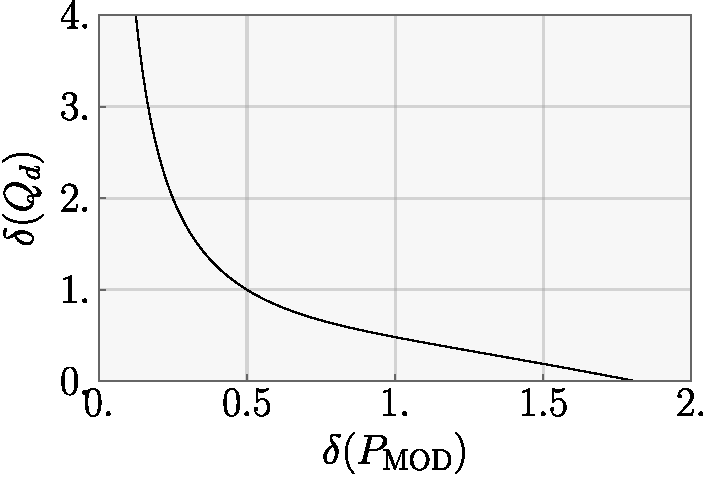
\includegraphics[width=0.8\textwidth]{ring-ur}
  \caption{The uncertainty region for the particle on a ring system, showing the curve obtained from the least eigenvalues of the operators $\Qd^2 + \alpha \MOD P^2$.}
  \label{fig:ring-ur}
\end{figure}

% further we can form the state
% \begin{align}
%   \xi_\alpha = \sum_{i =0}^{2n} x_i^\alpha \phi_{i-n}
% \end{align}
% where $\vec{x}^\alpha$ is the normalised eigenvector of $h_\alpha$ with least eigenvalue, and directly compute
% \begin{align}
%   \left(\braket{\xi_\alpha}{\MOD P^2 \xi_\alpha},\braket{\xi_\alpha}{ \Qd^2 \xi_\alpha}\right),
% \end{align}
% for various $\alpha$, giving a curve which must upper bound $b$, as well as approximate it as $n$ becomes large.
\subsection{Projective detection of interference}

We now proceed to the case (b) where the position on the second detector is recorded without identifying the endpoints of the interval, that is, distance between $\pi-\epsilon$ and $-\pi+\epsilon$ approaches $2\pi$ as $\epsilon\rightarrow 0$, acknowledging the fact that the maximum and minimum points of the spectrum of $\MOD P$ are $2\pi$ distance apart from each other.

As discussed above, the appropriate observable conjugate to $\MOD P$ now has continuous outcome set (in fact the whole of $\mathbb R$), and the solutions of the covariance system are characterised by dilation into $L^2(\mathbb R, \mathcal K_0)$ where it acts as the canonical position $Q$, and there is an isometry $\iota_0:\mathcal H_0\mapsto \mathcal K_0$. Applying the usual Fourier transform we write this as 
\begin{align}
UE(X)U^* = V^* (E^P(X)\otimes \id_{\mathcal K_0})V,
\end{align}
where $V:L^2([-\pi,\pi], \mathcal H_0)\to L^2(\mathbb R, \mathcal K_0)$ is an isometry for which $e^{ip Q\otimes \id}V=Ve^{ipQ_0\otimes \id}$, that is, $e^{ip Q\otimes \id}VI^* =VI^*e^{ipQ\otimes \id}$ where $I:L^2([-\pi,\pi], \mathcal H_0)\to L^2(\mathbb R, \mathcal K_0)$ is the isometry $(I\psi)(p) = \iota_0\psi_p$ for $p\in [-\pi,\pi]$ and zero elsewhere. Then $S:=VI^*$ commutes with $Q\otimes \id$ and hence must be decomposable in $L^2(\mathbb R,\mathcal K_0)$, that is, of the form $(S\psi)(p) = S_p\psi_p$, where $(S\psi)(p)=0$ for all $\psi$ for which $\psi_p$ vanishes on $[-\pi,\pi]$. The latter is only possible if $S_p=0$ outside $[-\pi,\pi]$, which implies that $V = VI^*I = SI$ has its range in $L^2([-\pi,\pi], \mathcal K_0)$, as in the periodic case. However, we now have $E^P(dp)=|e^{ipn}\rangle\langle e^{ipn}| dp$, that is, the spectral measure of the standard momentum with the continuum of ``eigenvectors'' $e^{ixp}$ respecting the Dirac delta normalisation, and since the outcome set is not equal to the dual group of $[-\pi,\pi]$, there are no spectral measure solutions - every possible path observable is a POVM with no projections in its range. Another way of saying this is that $VV^*$ cannot commute with all $E^P(X)$, which is explicit since $VV^*=SII^*S$ contains the spectral projection $II^*$ of $Q\otimes \id$.

In this case the resulting uncertainty measure reads
$$
\delta(E,\psi)^2 = \inf_{x_0\in \mathbb R} \int (x-x_0)^2 E_\psi(dx) = \inf_{x_0}\int x^2 E_{e^{-ix_0\MOD P}\psi}(dx),
$$
by covariance, and again this is finite exactly when $\psi$ is in the square integrability domain
$$
\{ \psi\mid \int x^2 E_{\psi}(dx) <\infty\},
$$
and in this case
$$
\delta(E,\psi)^2 = \int x^2 E_\psi(dx) - \langle \psi| E[1]\psi\rangle^2 = \var{E_\psi},
$$
where $E[1]$ is defined on the square integrability domain, provided the latter is dense. Now looking at the dilation we easily see that
$$
UE[1]U^* = V^*(P\otimes \id)V,
$$
where $P\otimes \id$ is unique selfadjoint extension of the corresponding algebraic tensor product operator. Since $(V\psi)(p)= S_p\iota_0\psi_p$ vanishes outside $[-\pi,\pi]$, and nevertheless needs to be absolutely continuous to make the uncertainty quantity finite,  $S_p\iota_0\psi_p$ must be absolutely continuous and hence vanish at the boundaries. Since each $S_p\iota_0$ is an isometry, this implies that $\psi_{-\pi}=\psi_{\pi}=0$. Hence the \emph{finiteness of the uncertainty quantity forces the Dirichlet boundary conditions if covariance holds.}

Now in general we can write 
$$
\delta(E,\psi)^2 = \|E[1]\psi\|^2 - \langle \psi| E[1]\psi\rangle^2 + N_E(\psi)
$$
where $N_E(\psi) := \int x^2 E_\psi(dx) -\|E[1]\psi\|^2$ is called the \emph{variance form} \cite{werner-screen-obs-1986}. Since $E$ is not projection valued, $N_E$ is typically not zero, in which case the ``intrinsic noise'' of the observable adds to the uncertainty. Hence from the point of view of sharp uncertainty relations it makes sense to restrict to observables with $N_E(\psi)=0$, which are called \emph{variance free} \cite{}. In this case the uncertainty quantity reduces to the form identical to the projection valued case, namely
$$
\delta(E,\psi)^2 = \|E[1]\psi\|^2 - \langle \psi| E[1]\psi\rangle^2 = \inf_{x_0} \| E[1]e^{-ix_0\MOD P}\psi\|^2,
$$
where we note that the domain is obviously invariant under $e^{ix_0\MOD P}$.

If we define $P_0\otimes \id$ as the operator with domain consisting of functions $\psi\in L^2(\mathbb R,\mathcal H_0)$ absolutely continuous in the strong sense of the existence of $\psi'\in L^2(\mathbb R,\mathcal H_0)$ for which $\psi_p = \int_{-\pi}^p \psi_p'dp'$ (where integral is Bochner, and we recall that $L^2$-functions are automatically integrable since the interval is bounded), and $\psi_{-\pi}=\psi_\pi=0$, we may also write
$$
E[1] = V^* (P_0\otimes \id) V.
$$
One can then easily check that $P_0\otimes \id$ is closed (same standard proof as with $P_0$ itself), and hence the variance-free condition implies that $E[1]$ is also closed, so the von Neumann theorem implies that $E[1]^*E[1]$ is selfadjoint on its domain as long as the domain of $E[1]$ is dense. Moreover, $VV^*P_0\otimes \id V\psi=(P_0\otimes \id) V\psi$ for any $\psi$ in the domain (by the stated invariance), and hence 
$$
E[1]^*E[1]\supset V^*(P_0^*P_0\otimes \id)V = V^*(H_0\otimes \id)V
$$
where $H_0$ is the usual ``particle in a box'' Hamiltonian. Consequently, for $\psi$ in this smaller domain, we obtain
\begin{align*}
  \delta(E,\psi)^2 &= \inf_{x_0} \expe{H_0}{Ve^{i x_0\MOD P}\psi}\\
                   &= \inf_{x_0} \expe{H_0}{e^{i x_0 Q_0}V\psi}\\
  \delta(\MOD P,\psi)^2 &= \expe{Q_0^2}{V\psi} -\langle Q_0\rangle_{V\psi}^2.
\end{align*}
The expectation term $\langle Q_0\rangle_{V\psi}$ reflects the fact that we do not have covariance for the other direction, that is, $P_0$ does not generate translations in the spectrum of $\MOD P$. Hence the uncertainty diagram will be more complicated in this case. However, if we restrict to the zero expectation subspace $\mathcal M := V^*(\xi_0\otimes \mathcal K_0)^\perp$ where
$\xi_0(p) =p$, we obtain the family of uncertainty relations
$$
\delta(E,\psi)^2+\alpha\delta(\MOD P,\psi)^2\geq c(\alpha)
$$
where $c(\alpha)$ is the bottom eigenvalue of the "particle in the box Hamiltonian" $H_0+\alpha Q_0^2$. The corresponding minimum uncertainty states are of the form $\psi = V^*(\varphi_\alpha\otimes\xi)$, provided that the range of $V$ contains at least of such product state, which happens when $V_pV_p^*\xi =\xi$ for almost all $p$, that is, the intersection of the ranges of $V_p$ is nontrivial.

Notice that there are easy examples where the domain is dense but does not contain any product vectors: for instance, if $V_p=V_-$ for $-\pi<p<0$ and $V_p=V_+$ for $0<p<\pi$ where the isometries $V_\pm$ have orthogonal ranges, then the domain consists of those vectors $\psi$ for which $\psi_p$ is absolutely continuous and vanishes at $-\pi$, $0$, and $\pi$. This case is variance-free since the derivative of $V_p\psi_p$ is just $V_p\psi_p'$, that is, is included in the range of $V$. It might be interesting to see if one can still get arbitrarily close to the minimum.

Hence in this case the form of the minimum uncertainty states is not so clearly fixed as in the periodic case. However, \emph{if we make the additional assumption that the minimum uncertainty must be reached}, that is, for at least one $\xi$ there is a $\psi$ in the domain so that $\varphi_\alpha\otimes\xi = VU\psi$ so $\varphi_\alpha(p) \xi = V_pU\psi_p$, that is, $U\psi_p= \eta_\alpha(p) V_p^*\xi$. Now $V$ need not be unitary so the isometry relation \eqref{orth} of the periodic case need not hold (so that integer translates of $\eta$ overlap), and continuous convolution is more appropriate - we have $\hat \psi(p) = \varphi_\alpha(p) \hat \eta(p)$ where $\varphi_\alpha$ is extended periodically over the whole $\mathbb R$, and $\hat \eta(p)$ is constructed so that $\hat\eta(p+n2\pi)= \langle n|V_p^*\xi\rangle$ for $p\in [-\pi,\pi]$. Now there is no constraint on the translates of $\eta$ being orthogonal, the inverse Fourier transform becomes convolution, and we end up with a continuous version of \eqref{minURC}:
\begin{align}\label{minUR2}
\psi(x) &= \int_{-\infty}^\infty dy\left[\int_{-\pi}^\pi dp \,e^{iyp}\varphi_\alpha(p)\right] \eta(x-y)
%&=\int_{-\infty}^\infty dy\left[\int_{-\pi}^\pi dp \,e^{i(x-y)p}\varphi_\alpha(p)\right] \eta(y)
\end{align}

\subsubsection{Uncertainty diagram}

Here we consider the case of the ``particle in a box'' system, the subset of $L^2([-\pi,\pi])$, of absolutely continuous functions, with absolutely continuous first derivatives. As indicated above the uncertainty quantity may only be finite if  $\psi(-\pi) = \psi(\pi) = 0$ are imposed, so we restrict to the subspace that respects these boundary conditions. On this space the operators position and momentum operators are defined in the usual way
\begin{align}
  (Q_0 \varphi)(x) &= x \varphi(x)\\
  P_0\varphi &= \varphi^\prime.
\end{align}
For any state in this space there is one with identical position and momentum variances, and momentum expectation value zero so, without loss of generality, we restrict our attention to the momentum expectation zero subspace. Obviously it is possible to construct states supported within $[-\varepsilon, \varepsilon]$ for any $\varepsilon>0$, similarly it is possible to construct states supported within $[-\pi, -\pi+\varepsilon]\cup [\pi-\varepsilon, \pi]$. We also note that given a state we can arbitrarily increase its ``momentum'' uncertainty, without changing the ``position'' uncertainty, for example by applying the operator $e^{i a Q_0^2}$ for some $a\in\R$. These considerations imply that the uncertainty region is entirely defined by the lower boundary function
\begin{align}
  b&:(0,\pi^2)\to \R^+\\
  b(x) &:= \inf_{\rho\in S(x)} \left\langle P_0^2\right\rangle_\rho,
\end{align}
where $S(x) = \left\{\rho\middle|\var{E^{Q_0}_\rho} = x \right\}$. There is a global minimum of this function $b\left(\frac{\pi^2}{3} -2\right) = \frac{1}{4}$, obtained by the ground state $\varphi_0$ of $H_0$. It is useful to note that the position expectation of $\varphi_0$ is zero, mixing (at the level of density operators) the minimising states with $\var{E^{Q_0}_\rho}\neq\frac{\pi^2}{3} -2$ with the projector $\ketbra{\varphi_0}{\varphi_0}$, one can show that $b$ is strictly decreasing on the open interval $\left(0,\frac{\pi^2}{3} -2\right)$ and strictly increasing on $\left(\frac{\pi^2}{3} -2,\pi^2\right)$. It is convenient to consider the two cases separately, we will refer to the region where $\var{E^{Q_0}_\rho} < \frac{\pi^2}{3} -2$ as the left hand side, and that where $\var{E^{Q_0}_\rho} > \frac{\pi^2}{3} -2$ as the right, in accordance with figure \ref{fig:box-ur}.

The concavity of $\rho\mapsto\var{E^{Q_0}_\rho}$ combined with the linearity of $\rho\mapsto \expe{P_0^2}{\rho}$ implies that on the right hand side the function $b$ is convex. We can therefore recover $b$ in this region from the convex conjugate
\begin{align}
  c(\alpha) &= -b^*(-\alpha)\\
  \label{eqn:rhs-conjugate}
            &= \begin{cases}\inf_{\rho}\expe{P_0^2}{\rho} + \alpha\var{E^{Q_0}_\rho}, & \alpha < 0\\
              \infty, & \alpha \geq 0
            \end{cases},
\end{align}
where we have set $b(x) = \infty$ for $x$ outside $\left(\frac{\pi^2}{3} -2,\pi^2\right)$, to restrict to the region of interest. We now show that, for negative $\alpha$, the infimum in \eqref{eqn:rhs-conjugate} is achieved by the ground state $\psi_\alpha$ of the operator $P_0^2 + \alpha Q_0^2$, to see this assume the contrary, there exists a state $\rho$ such that 
\begin{align}
  \expe{P_0^2}{\rho} + \alpha\var{E^{Q_0}_\rho} &< \expe{P_0^2}{\psi_\alpha} + \alpha\var{E^{Q_0}_{\psi_\alpha}},
\end{align}
rearranging, and noting that $\expe{Q_0}{\psi_\alpha} = 0$, we see
\begin{align}
  \expe{P_0^2 + \alpha Q_0^2}{\rho} - \alpha\expe{Q_0}{\rho}^2 &< \expe{P_o^2 + \alpha Q_0^2}{\psi_\alpha}\\
  \implies \expe{P_o^2 + \alpha Q_0^2}{\rho} &< \expe{P_o^2 + \alpha Q_0^2}{\psi_\alpha},
\end{align}
contradicting the definition of $\psi_\alpha$. Note that the assumption that $\alpha < 0$, resulting from restricting our attention to the right hand side, is critical in the derivation. 

We now turn out attention to the left hand side of \ref{fig:box-ur}, here we conjecture, but do not show, that the states with minimal uncertainty are once again the ground states of the Hamiltonian $P_0^2 + \alpha Q_0^2$, now with $\alpha >0$. If our conjecture is false then the curve we derive by solving the ground state problems will be an upper bound for the true boundary curve $b$. It is therefore interesting to look for a lower bound for $b$, an obvious choice is given by the isometry $I:L^2([-\pi,\pi])\to L^2(\R)$
\begin{align}
  (I\psi)(x) = \begin{cases}\psi(x),&x\in [-\pi,\pi]\\ 0, &\text{else}\end{cases}.
\end{align}
The usual $L^2(\R)$ position and momentum variances of $I\rho I^{*}$ are identical to the respective uncertainty quantities of $\rho$, the latter are therefore are subject to Heisenberg's uncertainty relation
\begin{align}
  \expe{P_0^2}{\rho} \var{E^{Q_0}_{\rho}} &= \var{E^{Q}_{I\rho I^{*}}} \var{E^{P}_{I\rho I^{*}}} \geq \frac{1}{4}.
\end{align}
In the limit of small position uncertainties this lower bound becomes tight, in the sense that
\begin{align}
  \lim_{x\to 0^{+}} x b(x) = \frac{1}{4},
\end{align}
which can be demonstrated by considering a sequence of truncated Gaussian states, equal to Gaussians with standard deviations $\sigma_n$ within the interval $[-\pi+\sigma_n, \pi-\sigma_n]$ and linearly interpolating between their values at $\pm (\pi-\sigma_n)$ and $\pm \pi$ outside as $\sigma_n \to 0$.

\begin{figure}
  \centering
  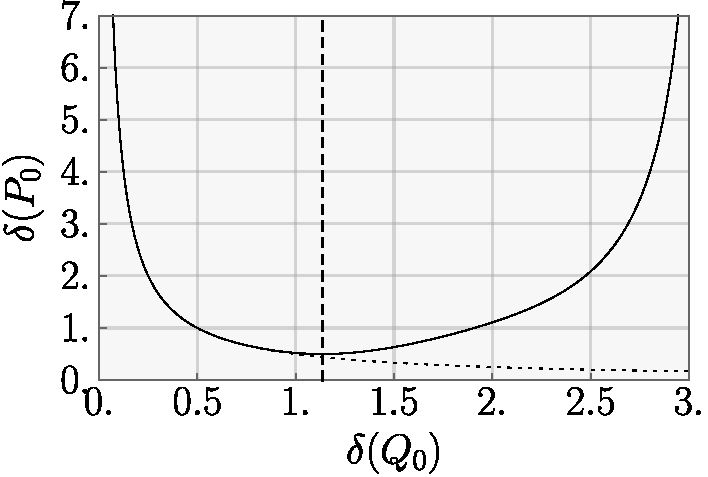
\includegraphics[width=0.8\textwidth]{box-ur}  
  \caption{The uncertainty region for the particle in a box system, showing the curve obtained from the least eigenvalues of the operators $P_0^2 + \alpha Q_0^2$ (solid curve), this is the exact boundary curve on the right hand side of the vertical line at $\sqrt{\frac{\pi^2}{3} -2}$ (dashed). On the left hand side the true curve lies between the solid curve and the canonical hyperbola (dotted). }
  \label{fig:box-ur}
\end{figure}

%$$ \inf_{x_0} \int_\mathbb{T} d_\mathbb{T}(x,x_0)^2 d\mu(x) $$



% We first note that given a state in this domain it is possible to shift the expectation value of the $P_0$ operator, while leaving 

% Before applying the Legendre transform method used above we must first show that the boundary of the uncertainty region 
% \begin{align}
%   b&:(0, \pi^2)\to \R^+\\
%   b&:x\mapsto \inf\left\{\expe{H_0}{\varphi} \middle|\, \expe{Q_0^2}{\varphi} - \expe{Q_0}{\varphi}^2 = x\right\},
% \end{align}
% is a convex function. Notice that $b$ has a global minimum at $a:= \frac{\pi^2}{3} - 2$
% $$
%   b(a) = \frac{1}{4},
% $$
% achieved by the ground state of $H_0$, which we will denote $\varphi_0$. Considering states of the form
% $$
%   \cos(\theta) e^{i\alpha}  \varphi_0 + \sin(\theta) \psi,
% $$
% where $\psi$ is a state on the boundary curve, and $a\in\R$ is chosen to ensure $\re\left(e^{ia}\langle\varphi_0|\psi\rangle\right)  \leq 0$, it is possible to show that the boundary curve is strictly decreasing on $(0, a)$ and strictly increasing on $(a, \pi^2)$. We now consider the convex conjugate of the boundary curve 
% \begin{align}
%   b^*(\alpha) := \inf_\psi\left(\expe{H_0}{\psi} + \alpha\left(\expe{Q_0^2}{\psi} - \expe{Q}{\psi}^2\right)\right),
% \end{align}
% defined for $\alpha\in\R$. Assuming differentiability we can recover the graph of $b^{**}$ as
% \begin{align}
%   \left\{\left(b^{*\prime}(\alpha),\, b(\alpha) - \alpha b^{*\prime}(\alpha)\right)|\, \alpha\in\R\right\}.
% \end{align}


% It is well known that the double convex conjugate of a function lower bounds it, further we note that 
%: the vector $e^{i\theta Q_d}\psi$ has again the form \eqref{basicstates} but with $c_n$ replaced by $c_n e^{i\theta n}$, and similarly $e^{-im \MOD P}$ effects the transformation $(c_n)\mapsto (c_{n+m})$ on \eqref{basicstates}. If we replace each sequence $(c_n)$ by the corresponding Fourier series $\sum_{n\in \mathbb Z} c_n \phi_n\in L^2[-\pi,\pi]$ where $\phi_n(\theta) = e^{in\theta}/\sqrt{2\pi}$, we recognise these transformations as the actions of the operators $e^{-i\theta P_0}$ and $e^{inQ_0}$ where $Q_0$ and $P_0$ are the usual multiplication and differentiation on $L^2[-\pi,\pi]$, the latter with \emph{periodic} boundary conditions. These then, of course, form the standard irreducible representation of the CCR on $\mathbb Z\times \mathbb T$, and we have reduced the interferometric CCR to its irreducible components.
%To summarise this precisely, the unitary operator $U: L^2[-\tfrac 12,\tfrac 12]\otimes L^2[-\pi,\pi]\to L^2(\mathbb R)$ defined by
%\begin{align*}
%U(\xi\otimes \eta) := \sum_{n\in \mathbb Z} \langle\phi_n|\eta\rangle e^{inP}\xi,
%\end{align*}
%effects the transformations
%\begin{align*}
%U^*Q_TU &= \id\otimes (-P_0), & U^*\MOD P U &= \id\otimes Q_0,
%\end{align*}
%where $L^2[-\tfrac 12,\tfrac 12]$ appears as a multiplicity space while the operators act nontrivially only on $L^2[-\pi,\pi]$.
%
%\begin{align*}
%U(\xi\otimes \eta) := \int dx \langle e^{ix\theta}|\eta\rangle e^{ixP}\xi,
%\end{align*}


%\section{The interferometric uncertainty relations}
%
%We now proceed to introduce an appropriate form of the interferometric uncertainty relations for the present setup, and show that the minimum uncertainty states are exactly mixtures of the basic states \eqref{basicstates} with certain fixed coefficients $c_n$ and arbitrary $\phi$. In particular, the form \eqref{basicstates} is forced by the requirement of minimal uncertainty.
%
%We begin with the fact that the relevant interferometric observables form a canonical pair with respect to the above CCR relations, and therefore any uncertainty relation should be based on this CCR. We use the approach of \cite{BKW}, but we need to take into account the reducibility of the interferometric representation, in contrast to the standard one discussed there. In order to present the UR we recall some basic facts from \cite{}: 
%
%
%The idea is to first choose translation invariant metrics for the outcome spaces of the two operators. In the case of the "slit number" outcome space $\mathbb Z$, we have two natural metrics: either we count how far two slits are from each other, or we simply settle for giving the minimal information telling whether they are distinct or not. The two metrics are given by
%\begin{align*}
%d_\Z(n,m) &=|n-m|, & d_{\Z}(n,m) =\delta_{nm}.
%\end{align*}
%For the outcome set $[-\pi,\pi]\simeq \mathbb T$ of $P_{\rm mod}$, there are two natural choices:
%\begin{align*}
%d_{{\rm arc}}(e^{i\theta},e^{i\theta'}) &:= |\theta\dot{-}\theta'|, \\
%d_{{\rm chord}}(e^{i\theta},e^{i\theta'}) &:=|e^{i\theta}-e^{i\theta'}|=\sqrt{2(1-\cos(\theta-\theta'))}.
%\end{align*}
%More generally, for a general translation invariant metric on $\mathbb T$ there exist a continuous positive symmetric $2\pi$-periodic \emph{potential} $\theta\mapsto V(\theta)$ such that $d(e^{i\theta},e^{i\theta'})^2=V(\theta-\theta')$. In the above two cases we have $V_{\rm arc}(\theta) = \theta^2$ (extended periodically from $[-\pi,\pi]$), and $V_{\rm chord}(\theta)=2(1-\cos\theta)$. In the following, fix a potential $V$ coming from a metric. (Only the periodicity, symmetricity and continuity are actually relevant.)
%
%We can now evaluate the relevant uncertainty quantities, taking into account the reducibility of the relevant CCR. Given any state $\psi\in \mathcal D(Q_d)$ we can write $\tilde \rho = {\rm tr}_{\mathcal H_0}[U^*\psi\rangle\langle U^*\psi|]$, so that $\E^{\Qd}_\psi=\E^{-P_0}_{\tilde\rho}$ and $\E^{P_{\rm mod}}_\psi=\E^{Q_0}_{\tilde\rho}$, and, consequently,
%\begin{align*}
%\ws{\Qd, \psi}&=\ws{-P_0,\tilde \rho}, & \ws{P_{\rm mod}, \psi}&=\ws{Q_0,\tilde \rho}.
%\end{align*}
%
%For a basic state $\psi$ of the form \eqref{basicstates}, we have $\psi= U(\xi\otimes  \varphi)$, and assuming standard metric on $\Z$, we get, independently of $\xi$, the uncertainty quantities
%\begin{align*}
%\delta(Q_T,\psi)^2&=\delta(P_0,\varphi)^2=\inf_{n_0\in \Z}\sum_{n\in \Z} n^2|\langle \varphi|\phi_{n+n_0}\rangle|^2\\
%&=\inf_{n_0\in \Z}\langle P_0e^{-in_0Q_0}\varphi|P_0 e^{-in_0Q_0}\varphi\rangle\label{UP0},\\
%\delta_{V}(P_{\rm mod},\psi)^2 &= \delta_{V}(Q_0,\varphi)^2\\
%&=\inf_{\theta_0\in [-\pi,\pi)} \int_{-\pi}^\pi V(\theta) |(e^{i\theta_0P_0}\varphi)(\theta)|^2d\theta\\
%&= \inf_{\theta_0\in [-\pi,\pi)} \langle e^{i\theta_0P_0}\varphi |V e^{i\theta_0P_0}\varphi\rangle,\end{align*}
%where $V$ also denotes the associated multiplication operator. Note that the former is finite as long as $\varphi$ is in the domain of $P_0$, that is, is absolutely continuous with $\varphi(-\pi)=\varphi(\pi)$ and the derivative is square integrable. According to \cite{BKW}, for an arbitrary pure state $\psi$, the uncertainty relation is thus of the form
%\begin{align*}
%&\delta(Q_T,\psi)^2+\alpha \delta_{V}(P_{\rm mod},\psi)^2 =
%\delta(P_0,\tilde \rho)^2+\alpha \delta_{V}(Q_0,\tilde \rho)^2\\
%&\geq \inf_{\varphi\in \dom{P_0}}\left(\delta(P_0,\varphi)^2+\alpha\delta_{V}(Q_0,\varphi)^2\right)\\
%&=\inf_{\varphi\in \dom{P_0^2}}\inf_{\omega\in \Omega} \langle W_0(\omega)\varphi|(P_0^2+\alpha V)W_0(\omega)\varphi\rangle\geq c_{V}(\alpha),
%\end{align*}
%where $c_V(\alpha)$ denotes the bottom eigenvalue of the operator $H_{V}(\alpha):=P_0^2+\alpha V$, see \cite{BKW} for more details. {\bf This does not include discrete metric yet!}. The last relation is saturated by certain specific \emph{minimum uncertainty state} $\varphi_\alpha$, which is even and has vanishing derivative at the boundary. The full interferometric URs are therefore given by
%\begin{equation}\label{intUR}
%\delta(Q_T,\rho)^2+\alpha \,\delta_{V}(P_{\rm mod},\rho)^2\geq c_V(\alpha)
%\end{equation}
%where $\rho$ is now an arbitrary (possibly mixed) state on $L^2(\mathbb R)$. While these lead to uncertainty diagrams identical to ones given in \cite{BKW}, the specific implication to the interferometric setting is that the \emph{minimum uncertainty states}, that is, those states which saturate the uncertainty relation \eqref{intUR}, are \emph{exactly} the convex combinations of the states of the form \eqref{basicstates}, where $\phi$ can vary while $c_n$ are the Fourier coefficients of the specific state $\varphi_\alpha \in L^2[-\pi,\pi]$, that is,
%\begin{equation}\label{minUR}
%V_\alpha\rho_0 V_\alpha^*,
%\end{equation}
%where $\rho_0$ is an arbitrary density matrix on $L^2[-\tfrac 12, \tfrac 12]$, and $V_\alpha:L^2[-\tfrac 12,\tfrac 12]\to L^2(\mathbb R)$ is the isometry given by $V_\alpha= \sum_{n\in \mathbb Z} c_n(\alpha) e^{-inP}$ where $c_n(\alpha)$ are the Fourier coefficients of $\varphi_\alpha\in L^2[-\pi,\pi]$.

%\section{Second measurement}
%
%Suppose now that we place a wire grating before the detector screen (see \cite{}), aligned with nodes of the typical interference pattern, so that the wires are located at points $(2m+1)\pi$ in the momentum space. The idea is that the wave function is then confined to each of the intervals, forcing the boundary condition $\eta(-\pi)=\eta(\pi) =0$, and also changing the relevant uncertainty quantification. In fact, due to confinement by the grating, the restriction to the interference pattern $\eta(p)$ to each of the intervals $2\pi m + [-\pi, \pi]$ should be considered separately, and hence the appropriate momentum observable (that is, position observable with respect to the first grating), should be considered as continuous rather than discrete, that is, the position at the slits is first transformed to the fourier space by way of the series, but then transformed back by way of an integral. Consequently, instead of the discrete $Q_d$, the probability density of the relevant position observable on the state \eqref{basicstates} is just 
%$$
%y\mapsto |\hat \eta(y)|^2 = \sum_{n,m} \overline{c_n} c_m \overline{s_n(y)}s_m(y),
%$$
%where $s_n$ is the sinc function. The states themselves are then best described by understanding the coefficients $c_n$ as expansion coefficients in the sinc function basis rather than the usual basis, that is, instead of
%$$
%\psi(x) = \sum_{n\in \mathbb Z} \langle \phi_n|\eta\rangle\, \phi(x-n) = \sum_{n\in Z} \langle s_n|\hat\eta\rangle \,\phi(x-n),
%$$
%where the Fourier transform is now understood in the full $L^2(\mathbb R)$, where $\eta$ is embedded as a function with support on the interval $[-\pi,\pi]$. The implication of this is that the observable is no longer projection valued, but corresponds to a POVM. Now given the restriction
%$$
%\sum_{m} c_{2m}=\sum_{m} c_{2m-1},
%$$
%which defines a dense subspace of $L^2(\mathbb R)$, we are left with only the states vanishing at the boundary, and these are conveniently lying in the domain of the version of the operator $-id/(d\theta)$ where the boundary condition is the vanishing of the function at $-\pi$ and $\pi$.


%We only consider the case where the incident wavefunction is odd, that is, $c_n=-c_{-n}$. In this case only the combinations $\phi_{n}-\phi_{-n}$ appear for odd values of $n$, and, consequently, we can use the basis of sine functions $\psi_n = \sin((k+1)(x-\pi)/2)$ instead. This happens to be the eigenbasis of the ``particle in a box'' Hamiltonian 
